In this part of the documentation, our goal is to explain how ART handles colour values, spectra, light, and the attenuation of light. Each of these types has different properties, but the four categories are not entirely orthogonal, either. \emph{Light} and the \emph{attenuation of light} are counterparts, have an exact physical meaning. \emph{Spectral data} are directly measurable wavelength-dependent physical quantities, while \emph{colour values} are merely correlates of human perception. At various points in a physically based rendering system, one wants to be able to work with all four of these quantities, so they have to exist alongside each other. As they do share some similarities, we sometimes collectively refer to them as the \textbf{CSLA} data types (Colour, Spectra, Light, and Attenuation). An overview of the main data types in the current CSLA system is shown in figure~\ref{fig:csla_subsystem}.

ART is not new software: over the years, it went through several evolutions with regard to how it handles such matters. In part, this happened because we still had to figure out how to do some of these things -- for some aspects of the system, there was no real prior art to guide us. And the first attempt at designing any new, complex system is rarely a total success. So an explanation of the  functionality currently found in ART requires a brief historical outline how its spectral rendering sub-system evolved.

This is particularly true since its rather gradual, evolutionary and protracted development led to ART 2.x still containing some features that would, strictly speaking, no longer be necessary for ART in its current form. For some tasks within the rendering workflow, these old features -- and in particular, the ISR switching architecture discussed later -- are still useable as they are, though, which is why they were retained. To keep this document reasonably brief, we do not go into great detail about non-spectral aspects of ART development: considerably more was achieved with early versions of ART in terms of research output (for instance, with regard to procedural modelling, and global illumination) than we mention here. 

If you want to directly jump to an outline of how current ART handles spectral path tracing, you can directly proceed to section~\ref{sect:currentart}.

\chapter{The Evolution of Spectral Rendering in ART}
\label{sect:arthistory}
\section{Early ART: the 0.x series}

ART has its origins in an age when a lot of current mainstream graphics technology was either still unknown, or at least  in a very experimental stage: its development started in 1996, as a standard RGB Whitted ray tracer. Initially, the project was aligned with the research interests of Robert F. Tobler, or \command{rft}, as he was professionally known via his lowercase initials. He was the founder of the project, and for around 6 years, also its chief architect. At the time he started to develop ART, he was an assistant professor at the Institute of Computer Graphics at Vienna University of Technology, and needed an environment to try out his research ideas. He worked on novel procedural modelling techniques, use of innovative data structures in graphics, advanced scene graph semantics, CSG modelling, shading languages, and stochastic radiosity techniques: physically based rendering was actually not one of his main interests at the time. For this work, \command{rft} needed a software framework: and in 1996, the only sensible option was to roll one's own renderer, as no open source software existed which would have been remotely useful for such purposes. From the very get-go, the ART source tree featured its characteristic mix between ANSI C and Objective-C which is discussed in section~\ref{sect:mixingCandC}.

\begin{figure}[htbp]
\begin{center}
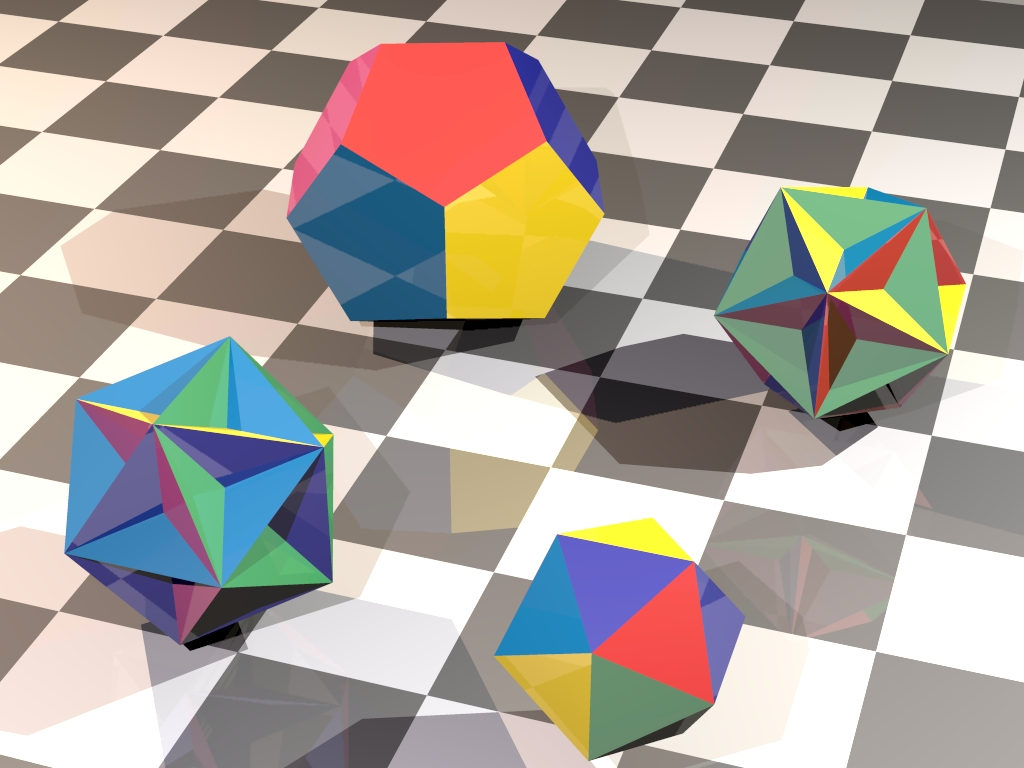
\includegraphics[width=.3\linewidth]{Images/Old_ART_Platonics.jpg} 
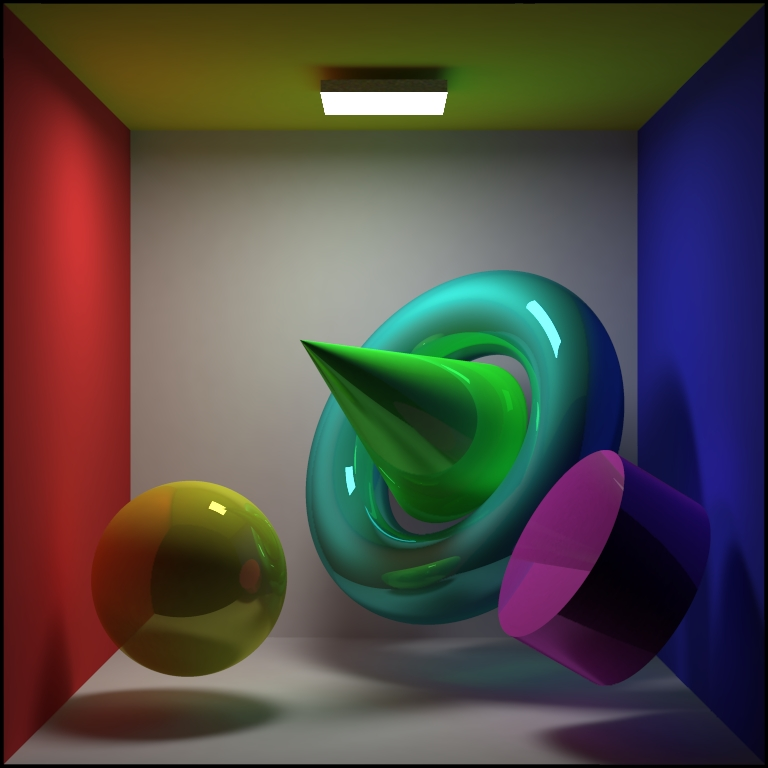
\includegraphics[width=.225\linewidth]{Images/Old_ART_Quadrics.jpg} 
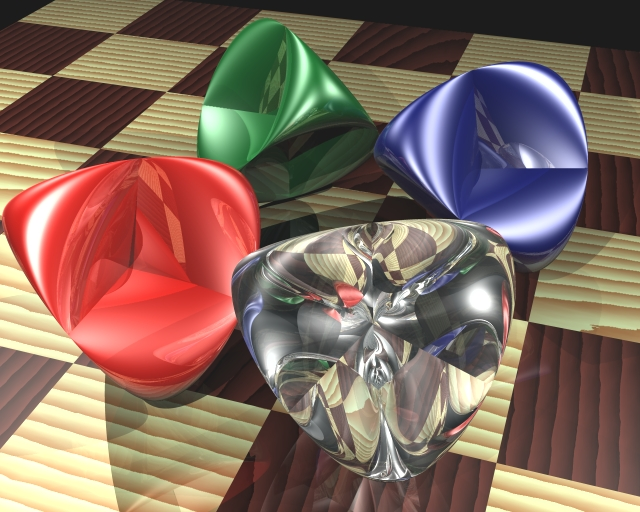
\includegraphics[width=.2825\linewidth]{Images/Old_ART_Steiners.jpg} 
\end{center}
\caption{
\label{fig:old_art} 
Images rendered with 0.x versions of ART in the approx.~timeframe 1996-2002. When handled correctly, even a fairly primitive renderer like a Whitted ray tracer could yield visually rich images. Note, however, that all reflections are perfect mirror reflections, or fake Phong highlights. The global illumination effects seen in the middle image were the result of a hybrid approach which pre-computed global illumination via stochastic radiosity: the final gather was still done via Whitted ray tracing. Also note how the rightmost image shows that even the 0.x series of ART already had a procedural shading language, which in this example was used to create the woodgrain texture on the chessboard.
}
\end{figure}

As a consequence of this background, the first versions of ART were heavily geared towards \command{rft}'s personal research topics. Visualisation of scene graphs was for a long time done via a comparatively primitive algorithm: classic Whitted ray tracing, \ie old school ray tracing which is only capable of dealing with perfectly diffuse surfaces and perfect mirrors, plus fake glossy highlights on Phong surfaces. Such a renderer does not compute global illumination, although GI could, at least in some sub-versions of early ART, be added via a stochastic radiosity pass. Point light sources were the norm; figure~\ref{fig:old_art} shows a few example images. 

\section{Middle Ages: ART 1.x}

Spectral rendering, including the ability to store spectral images in a special lossless HDR image file format called \filename{artraw} (see section~\ref{sect:propformats}), was added to the system starting around the year 1998. Polarisation support followed around the year 2000, and the initial version of \filename{artraw} was developed to store polarisation information: before that, Greg Ward's LogLuv HDR TIFF variant had been used as intermediate storage format between renderer and tonemapper. Bi-spectral capabilities were added in 2001. Due to the inclusion of polarisation and bi-spectral capabilities, the conceptual split between light and attenuation values discussed in section~\ref{sec:lightandattenuation} had to be introduced in the codebase around this time: this feature is conceptually one level above the actual spectral representation, and has been retained in more or less unchanged form since then.

By then, the system had become a collaborative effort between several persons at the institute, although \command{rft} was still the overall maintainer and designer. The version number was pushed to above 1 at some point after 2002, but ART was not publicly released then. This was mainly due to still being rather unfinished, and poorly documented: but there was always also a recurring theme of \emph{"we will do one more paper based on some advanced feature that no other renderer has, and then we will make it Open Source"}. Of course, by the time that particular paper had been done, there was always another one on the horizon, as convenient reason not to invest the considerable overhead needed to clean up the toolkit for release. After all, researchers are in the business of producing papers, not Open Source software.

When the ART version number was pushed to 1.x, \command{rft} had already left the institute, to work as senior researcher at the then newly opened VRVis graphics research centre. Although this centre is also located in Vienna, its research focus has always been more oriented towards interactive graphics, so an offline renderer like ART was not a research priority there. At VRVis, \command{rft} started work on an entirely new interactive rendering system called \emph{Aardvark}, which has  semantically very rich modelling capabilities: it has a number of features which are still ahead of its time even now, and which is still in production use there. As a result of \command{rft} having this new project on his hands, responsibility for ART changed over to the current maintainer, Alexander Wilkie, around 2003. Until 2008/2009, the 1.x series of ART continued to be used for work on publications by a sub-group at the Institute for Computer Graphics and Algorithms at Vienna Tech. 

In spite of spectral (and later even bi-spectral) rendering capabilities having been added, ART also continued to offer the functionality of rendering in colour space. This hybrid nature persisted through all ART 1.x versions: you could compile ART 1.x as an RGB renderer, but also as a spectral renderer which used $n$ fixed bins for its spectral representations, with 8, 16, 45 and 450\footnote{The mode with 450 spectral bins was intended for reference renderings with 1nm sampling distance across the visible range. It was never really used in practice, though, due to being extremely slow, and memory hungry. ART 2.x dropped this option.} bins being offered. Polarisation support was also a compile time option, and orthogonal to the chosen spectral resolution. This fact was cleverly hidden from the user: the actual renderer 'executable' \command{artist} was in fact a shell script, which picked the right executable (RGB, spectral, polarisation capable or not,...), based on user preferences. This was a hack, and made debugging quite difficult: but it did work reasonably well, and allowed one to compare the results obtained with different spectral sampling densities. Internally, a pseudo-polymorphic data type called \command{Colour} was used in all places that could refer to either a colour value or a spectrum: this macro placeholder was replaced with an appropriate structure at compile time\footnote{While this way of doing things is perfectly valid when working with ANSI C (at least purely from a technical viewpoint), the macro replacement of all instances of \command{Colour} was one of the reasons why ART 1.x executables were a pain to debug.}. The way this was done was via a simple \command{\#define}, such as \eg

\begin{verbatim}
#define Colour  Spectrum8
\end{verbatim}

to make all instances of \command{Colour} an 8 channel spectrum: \source{Spectrum8} was a simple ANSI C structure which contained 8 floats. This had the advantage that all instances of \command{Colour} could be statically allocated, as their size was known at compile time: no dynamic allocation and de-allocation of this internal representation of colours and spectra was needed. Due to the performance considerations discussed in section~\ref{sect:mixingCandC}, the representations of spectra and colours one could choose were implemented as low level C structures, and not ObjC classes, where polymorphism would have been available via the language.

\begin{figure}[htb]
\begin{center}
\includegraphics[width=.7\linewidth]{Images/Old_Spectral_Workflow.pdf} 
\end{center}
\caption{
\label{fig:old_spectralworkflow}
The logic of the fixed representation spectral workflow in ART 1.x, and early 2.x alpha. There is a wide range of input data that can be used in a scene description: but it all gets converted to a specific \emph{Internal Spectral Representation} (ISR), which is used during all computations, and which gets written into the result image. In this example, all input data is being reduced to the \command{Spectrum16} data type: as result, this data type exclusively gets used during rendering, and the resulting \filename{artraw} image also contains such data. The advantage of such an architecture is that no conversions, interpolation or splatting is being done during path tracing: all data is converted to the used ISR prior to rendering, and results are directly written to disk. Compare this to the current workflow, shown in figure~\ref{fig:spectralworkflow}.
}
\end{figure}

But "nailing down" the main spectral representation to one particular low-level C type (as opposed to a fancier solution with polymorphic ObjC types) was not only about performance: it was also implicitly about the data handling logic of the renderer itself. Polymorphism in the data structures which are used to describe colour or spectra in the core of the renderer is only useful if it serves a semantic purpose: but as figure~\ref{fig:old_spectralworkflow} shows, the logic of ART 1.x (and early 2.x) was to reduce all input data to a given internal representation on start up anyway, to avoid conversion calculations during the actual rendering loop. For this sort of logic, a simple C structure is perfectly sufficient, and actually desirable.

How was this \command{Colour} datatype used: the following code snippet is taken from Lambert surface material code of an ART 1.x version. First, the subnode which contains the actual colour (or spectral information) attached to the surface material is queried to return a \command{Colour} value for the given \command{hitInfo}, \ie a data structure which contains information on where the ray in question hit the object. The information in the \command{hitInfo} is \eg used to compute procedural texture results. Then, this \command{Colour} value is used to construct an \command{ArFilter} value, which is returned as the result of the method call: 

\begin{verbatim}
Colour  reflectionColour;
    
[ COLOUR_SUBNODE getColour: hitInfo : & reflectionColour ];

arfilter_c_init_nonpolarizing_f( & reflectionColour, outReflectionFilter );
\end{verbatim}

Note that \command{ArFilter} is the ART 1.x name for what is now known as \command{ArAttenuation} values (see section~\ref{sect:attenuation}). The idea behind the old name was that the information contained in it usually describes a \emph{filtering} of light\footnote{"Filtering" in the sense of light falling through a coloured filter, and being attenuated by it.}. This was later changed, as the term "filter" already has a set meaning in mainstream Computer Graphics, so ART 1.x usage of the term was needlessly confusing.

Overall, the \command{Colour}-based, "hardwired" hybrid colourspace and spectral ART 1.x worked reasonably well, with the only special cases in the codebase being caused by the distinction between polarising and non-polarising forms of the renderer. But unfortunately, after over ten years of not always perfectly guided development, the core software structure of ART 1.x, with its various idiosyncrasies, became more or less un-maintainable around 2007. Even worse was the fact that after a certain point, no single copy of the system which had all components in functional state existed. No version control for sources had been in use at the Vienna institute (in hindsight, this was a huge mistake), so merging was a manual process, and rarely done. Every research effort spawned a forked source tree, and a number of interesting research results were lost -- at least with regard to the source code used to generate the results found in the corresponding paper -- when such sub-versions of ART eventually were discarded along with old computers in the lab. In addition to all this, in spite of it working reasonably well when handled carefully, the hardwired spectral switching technique via \command{\#define} was clearly not an adequate long-term solution from a software engineering viewpoint: but as it was so ingrained in the system, nothing short of a major re-write would yield a useable alternative.


\section{Renaissance: early ART 2.x alphas}

In 2008, the maintainer of ART moved to Charles University in Prague. By then, several physically based open source rendering systems had been published, most notably the seminal \command{pbrt}. However, none of the available systems were (bi-)spectral, or had polarisation capabilities. Nor did any system use a stable and documented spectral image file format. As these topics continued to be of considerable research interest to the maintainer, and as such capabilities are very hard to retro-fit into other more mainstream rendering systems (such as \command{pbrt}), the decision was made to keep ART around, and to start a complete overhaul of the system. However, this overhaul went along a gradual path: with regard to spectral rendering, early alpha versions of ART 2.x were essentially a more sane and stable re-implementation of the dual colourspace/spectral capabilities seen in the ART 1.x series, and which are illustrated in figure~\ref{fig:old_spectralworkflow}. It was only the later 2.x alphas which dropped the capability to render in colourspace, and which switched to the current pure spectral rendering model that is discussed in section~\ref{sect:currentart}.

\subsection{Internal Spectral Representations}
\label{sect:CCTs}
It was not before the complete re-write that was to become ART 2.x that the \emph{internal spectral representation} (ISR for short) of colour values and/or spectra became something you could actually switch in a running instance of ART. In the early alphas of 2.x, a polymorphic data type that can resolve to either form during runtime was introduced: the structure which is now called \command{ArSpectrum}. Admittedly, \command{ArSpectrum} is not a perfect name for this data type (just like the name for its exact counterpart \command{Colour} in ART 1.x was not) -- after all, the content of this data structure can also be a colour value, and not just a spectrum. But the English language seems to lack an expression which succinctly describes both types of data at the same time.

Technically, \command{ArSpectrum} is a struct that contains a single \source{void *} pointer which references the actual data. The actual data can, in turn, be one of the ISRs supported by ART. Because of this, instances of \command{ArSpectrum} can only be dynamically created and deleted via their associated \command{spc\_alloc()} and \command{spc\_free()} functions. Static instances of \source{ArSpectrum} do not make sense, and do not work. All functions that operate on \command{ArSpectrum} instances are re-directions to the appropriate functions for the "native" content of the \command{ArSpectrum} struct. Figure~\ref{fig:arcolour} shows an overview of this.

\begin{figure}[htbp]
\begin{center}
\includegraphics[width=.5\linewidth]{Images/ArSpectrum.pdf} 
\end{center}
\caption{
\label{fig:arcolour} 
Graphical illustration of the \source{ArSpectrum} wrapper data type. The \source{void} pointer inside the struct can point to any of a number of ISR types (listed on the right). Functions that operate on \source{ArSpectrum} arguments use a function pointer that is stored in the \source{ART\_GV} protected global state, and changed accordingly when the ISR is being switched, to call the correct function to operate on the \source{void *} contents of the struct. In effect, this approach is a form of object oriented programming and encapsulation, only done via pure C and function pointers for performance and portability reasons.
}
\end{figure}

The following ISRs are currently available in ART: see figure~\ref{fig:art_isr_ranges} for an illustration of their respective ranges. If you want to compare their performance, render the Macbeth colour charts found in the gallery section.

\begin{enumerate}
\item \textbf{\source{ArSpectrum8}}, command line flag \textbf{-s8v}: an 8 band visible range spectrum with 40nm spacing. Intended as reasonable option in terms of \source{artraw} file size, but which still delivers quite passable colour accuracy. This setting is the default.
\item \textbf{\source{ArSpectrum11}}, command line flag \textbf{-s11e}: an 11 band spectrum with 40nm spacing, which covers both the near UV as well as the visible range. The bands in this spectral type correspond to the bands used in the Hosek sky dome model, and were originally defined for this purpose. Suitable for extended range data which does not have any sharp spectral features.
\item \textbf{\source{ArSpectrum18}}, command line flag \textbf{-s18v}: an 18 band visible range spectrum with 20nm spacing. A higher accuracy option for visible range images.
\item \textbf{\source{ArSpectrum46}}, command line flag \textbf{-s46e}: a 46 band spectrum with 10nm spacing, which covers both the near UV as well as the visible range. A high-accuracy counterpart to \textbf{s11}, which can also be used for reference images in the visible range.
\end{enumerate}

This particular selection of ISRs is only weakly hard-coded into ART -- adding more would be a fairly small effort. 

\begin{figure}[htb]
\begin{center}
\includegraphics[width=.8\linewidth]{Images/ART_ISR_Ranges.pdf} 
\end{center}
\caption{
\label{fig:art_isr_ranges} 
Spectral ranges of the current ART ISRs, plus the internal \textbf{s500} type: the red vertical lines denote what can be seen as the "main visible range". The CIE XYZ standard observer functions are defined to beyond 800nm, but only have tiny values beyond 700nm. For instance, the cut-off of \textbf{s8v} at 700nm is motivated by the fact that for equal energy illumination, and the 1932 CIE XYZ primaries, the energy above 700nm accounts for the following percentages in an XYZ triplet: $(0.15\%,0.06\%,0.00\%)$. \textbf{s18v} adds two bands that go to 740nm, which accounts for $(0.14\%,0.05\%,0.00\%)$ of the remaining energy, \ie practically the entire missing energy. \textbf{s500} is intended as an internal catch-all datatype, and as such has to go beyond all actual spectral ranges found in \source{artraw} images.
}
\end{figure}

Once they started up, the early ART 2.x alphas used one of these ISR types for all its internal calculations that involved basic "colour or spectral values", exactly as ART 1.x had used the \command{Colour} data type. All user-specified data were converted to the accuracy of the currently active ISR prior to rendering, and images generated while running in a particular mode were saved in their native ISR form, so that no data is destroyed after rendering (see section~\ref{sect:propformats} on \filename{artraw}, which is the file format that is capable of storing whatever ISR data is put into it). Figure~\ref{fig:old_spectralworkflow} gives a schematic of this process. Switching the ISR involves changing all the function pointers which are used to manipulate the contents of \command{ArSpectrum} instances. Also, certain in-built constants (such as the values for black and white, or zero and unit radiance/reflectance, respectively) have to be re-created to match the current ISR. The place where one can find the source for all this is the \command{ColourAndSpectra} library in the Foundation part of ART.

Because of the low-level nature of this switching process, it is not feasible to switch the ISR once a scene has been loaded, or during rendering. If the user specifies that a file be rendered in a particular ISR that differs from the current standard of \command{ArSpectrum8}, the first thing the \command{artist} command-line renderer does is to switch ISR, before doing anything else. The command line options for the \command{artist} renderer which switch to a particular ISR are \option{-rgb}, \option{-s8}, \option{-s11}, \option{-s16} and \option{-s45}, respectively.

The approach to directly use the ISRs during path tracing calculations, and to reduce all data to the ISR on loading, was ultimately dropped for two reasons:

\begin{enumerate}
\item As the development of physically based rendering progressed, it made less and less sense to retain the colourspace rendering capabilities which ART 1.x had had.
\item It became clear that fixed width spectral representations do have their uses, but not in the core of a renderer. There, either monochrome or Hero sampled spectra are much more appropriate.
\end{enumerate}

As we will see in the next section, ART 2.x actually retains the capability of being switched to a particular ISR. However, internally, mono or Hero sampling is used for all spectral data, and the choice of ISR now only affects the spectral sampling rate of the output image. The early ART 2.x alphas were, in spite of their transient nature, still used for work on a number of publications during the 2010-2016 timeframe. 

\section{Modernity: Spectral Path Tracing in Current ART 2.x}
\label{sect:currentart}

Low level handling of spectral quantities in ART path tracing is internally done via the \emph{Hero wavelength sampling} approach which was first demonstrated in the Manuka renderer of Weta Digital: as of 2018, this appears to be the current state of the art in spectral rendering. The path tracer of ART 2.x is no longer able to internally work in colour space, which from the viewpoint of physical correctness is hardly a negative thing: all path tracing is now exclusively done with spectral data. An overview of the new workflow can be seen in figure~\ref{fig:spectralworkflow}.

\begin{figure}[htb]
\begin{center}
\includegraphics[width=.7\linewidth]{Images/Spectral_Workflow.pdf} 
\end{center}
\caption{
\label{fig:spectralworkflow}
The current spectral workflow in the ART path 2.x tracer. Note that the user still selects an ISR (underlaid in purple), like in the ART 1.x workflow shown in figure~\ref{fig:old_spectralworkflow}: however, this now only affects the spectral resolution of the output image. For path tracing, all other spectral data is actually \emph{upsampled} to an internal form with 1nm spectral resolution. The advantage of this is that random wavelength sampling can directly grab any wavelength bin, and use it without any interpolation or further processing. The downside of this technique is memory usage, which is typically not an issue unless the scene contains image maps. Results of the core rendering loop are splatted into the result \filename{artraw}. Note that this result file can also contain colour space data, if the user selects this. Also note that the inclusion of polarisation information is orthogonal to the \source{ArSpectrum} type: the actual data stored in an \filename{artraw} are \source{ArLight} values, which can be either plain or polarising. See figure~\ref{fig:csla_subsystem} for an overview. 
}
\end{figure}


Internally, the data type \command{ArSpectralSample}, with its accompanying type \command{ArWavelength} to describe the sampling wavelength(s), is now being used for all spectral samples taken by the path tracer. Once an estimate has been obtained, these samples are splatted into the result \filename{artraw}. Hero sampling is conceptually simpler in a number of ways than the previously used fixed-width spectral representations: and it is also faster, more suited for polarisation rendering, and less biased than the old techniques. Hero sampling is being used by default: but for debugging and verification purposes, ART can actually be switched to "monochrome mode", where only a single wavelength is traced. The workflow shown in figure~\ref{fig:spectralworkflow} remains the same if this is done.

On a higher level, ART 2.x continues to use the concept of light and attenuation values discussed in section~\ref{sec:lightandattenuation}, and which was first introduced in ART 1.x. For use within the path tracer, the corresponding sample types \source{ArLightSample} and \source{ArAttenuationSample} were introduced.
 
Once the switch to Hero rendering was complete, the entire switching machinery behind the polymorphic \command{ArSpectrum} data type from the early 2.x alphas could theoretically have been removed from ART, as it is not needed for direct rendering purposes anymore. However, the notion of selecting a "master ISR" which all spectral data can default to was actually retained: mainly because the sub-system was already there, well tested, and stable. It was reduced in importance, though, as can be seen from figure~\ref{fig:spectralworkflow}: it now only affects the resolution of the output image. In principle, the infrastructure of being able to switch the entire \command{ArSpectrum} infrastructure between specific ISR types is now considerable overkill for just selecting a data type used for \command{artraw} content: as such, this sub-system would not have been written "from scratch" the way it is for the purpose it is being used for now. But as long as it does not get in the way of new functionality (and it is hard to see how it would do that), it stays in the toolkit.

\chapter{Light and Attenuation}
\label{sec:lightandattenuation}

As stated before, due to having to deal with polarisation and bi-spectral data, ART internally has to make a distinction between light values (\source{ArLight} structs) and light attenuation values (\source{ArAttenuation}
structs). There are also corresponding types for single or Hero wavelength samples taken from either. In this section, we explain some of the internal workings of these data types, and the relationship between them. We briefly discuss naming, start with a general overview of \source{ArAttenuation}, and then discuss the issues specific to the polarisation support within ART.

\begin{figure}[htb]
\begin{center}
\includegraphics[width=.7\linewidth]{Images/CSLA_Subsystem.pdf} 
\end{center}
\caption{
\label{fig:csla_subsystem} 
Overview of the respective contents of all the switchable data types of the CSLA subsystem (\source{ArSpectrum}, \source{ArLightSample}, \source{ArLight} and \source{ArDirectAttenuation}) for the various operation modes of ART. \source{ArSpectrumXX} stands for any of the concrete spectral ISRs, such as \eg\source{ArSpectrum45}.
}
\end{figure}

\section{The \source{ArAttenuation} Data Type}

One of the physical effects ART is designed to handle is fluorescence: this means that apart from directly attenuating the incident energy, any light-matter interaction can also potentially transfer energy from one waveband to another. So for the old ART 1.x renderer, and the early 2.x alphas, which both worked on entire spectra at once, a counterpart to \source{ArLight} which was capable of encoding this energy-shifting behaviour was needed. The path tracer in ART 2.x does not actually use \source{ArAttenuation} anymore, and instead works with wavelength-sampling \source{ArAttenuationSamples}, and explicit wavelength shifts to handle fluorescence: for such surfaces, it also integrates over the wavelength shifting dimension. So technically speaking, the \source{ArAttenuation} data type described here is no longer needed: but as the code was functional, it made no sense to explicitly delete it.

\subsection{Naming Conventions: Attenuation \vs Reflectance}
\label{sect:attenuation}
In ART, we use the term \emph{attenuation} (of light) as a general term for the changes in intensity that light undergoes upon interaction with matter. In most rendering systems, expressions like \emph{reflectance} are used for this sort of quantity. However, in ART, the attenuation data type is intended to encode \emph{all} interactions of light with matter, and this goes beyond mere reflectance: scattering events (\eg Rayleigh scattering in the atmosphere) are one example of this. The \source{ArAttenuation} data type also encodes fluorescence effects, which involve energy transfer between different wavelengths -- yet another concept that goes beyond normal reflectance.

\subsection{\source{ArAttenuation} Contents}

In order to handle fluorescence, an \source{ArAttenuation} struct contains two main components:

\begin{enumerate}
\item an \source{ArCrosstalk} structure, which describes the frequency/colour band crosstalk found in fluorescent materials, and
\item an \source{ArDirectAttenuation} structure, which is the classical reflectance value. 
\end{enumerate}

Figure~\ref{fig:arattenuation} gives a graphical overview of this. Notable points are that the direct attenuation (but only that -- the fluorescence described by the crosstalk is a non-polarising phenomenon) can be switched between a polarisation-aware form and a plain one, and that flags are used to make certain operations more efficient.

\begin{figure}[htb]
\begin{center}
\includegraphics[width=.6\linewidth]{Images/ArAttenuation.pdf} 
\end{center}
\caption{
\label{fig:arattenuation} 
\source{ArAttenuation} contains two components, the crosstalk data structure, and the direct attenuation. The \source{ArDirectAttenuation} struct switches between plain and a polarisation-aware mode and, like \source{ArLight}, expands to a single \source{ArSpectrum} value for the non-polarising mode. The fluorescence crosstalk is always just an array of float values, since it is a purely non-polarising phenomenon.
}
\end{figure}

\section{\source{ArLight}}
Compared to \source{ArAttenuation}, \source{ArLight} is a rather simple data type. For a plain rendering system without
polarisation support it just contains a single \source{ArSpectrum} instance: nothing more than a colour value or a spectrum is needed to describe a radiance value. If the system is switched to polarisation-aware mode, it contains a C structure with 4~elements of type \type{ArSpectrum} to encode the 4~components of the Stokes Vector, as well as a single reference frame.

\begin{figure}[htb]
\begin{center}
\includegraphics[width=.9\linewidth]{Images/ArLight.pdf} 
\end{center}
\caption{
\label{fig:arlight} 
\source{ArLight} contains a \source{void} pointer to allow a switch between plain and polarisable data structures. The plain light data structure is an \source{ArSpectrum} value, while the polarisation-aware version, \source{ArSVLight}, contains a Stokes Vector representation and a reference frame.
}
\end{figure}

Like \source{ArAttenuation}, \source{ArLight} values are no longer directly used during the path space computations of ART. But unlike the attenuation struct, it still has a very important purpose: \source{artraw} result images have pixels which are \source{ArLight} structs. Each \source{ArLightSample} which is computed by a path is splatted into the result \source{ArLight} for the pixel it belongs to.

\section{Polarisation Support}

Polarisation-aware routines for the manipulation of light and reflectance data are significantly more computationally costly than their plain counterparts. In practice, this means that it is infeasible to permanently activate this sort of functionality in a general purpose rendering engine such as ART. So in order to support rendering with polarised light, both light and attenuation data have to be switchable between plain and polarisation-aware versions. By default, \source{artist} runs in plain mode, and for those executables where such a functionality makes sense, the polarisation mode can be activated via the \source{-p} command line flag.

\begin{figure}[htbp]
\begin{center}
\includegraphics[width=.7\linewidth]{Images/C_Structures.pdf} 
\end{center}
\caption{
\label{fig:c_structs} 
The two polarisation-aware data structures \source{ArSVLight} and \source{ArMMDirectAttenuation} shown side by side. Note that the Stokes Vector structure has a single reference frame, while the one for the Mueller Matrix has two.
}
\end{figure}

To make this switching possible, the remaining other CSLA types like \source{ArLight} \ea are, exactly like \source{ArSpectrum}, also shell structures with a single \source{void} pointer inside: their inner workings, and their initialisation, are practically identical those of \source{ArSpectrum} discussed in section~\ref{sect:CCTs}. The similarities include the fact that the switch to the desired mode has to be made very early during the start-up sequence of ART, and that the mode cannot be easily changed once the system is running. A difference is that the switch they perform is not done between several ISRs, but between plain versions of the data structure in question (\source{ArPlainLight} and \source{ArPlainDirectAttenuation}, which are both just \source{ArSpectrum} in disguise), and their polarisation-aware counterparts (\source{ArSVLight} and \source{ArMMDirectAttenuation}, where SV stands for "Stokes Vector", and MM for "Mueller Matrix"). Figure~\ref{fig:csla_subsystem} shows a diagram which explains the contents of each of the top-level structures for the various operation modes of ART.

\section{Using CSLA Values in ART Rendering Code}

Contrary to what the somewhat involved preceding paragraphs might suggest, usage
of such data types within ART is very straightforward, since a considerable effort is made to
conceal all the inner workings of the switching CSLA system. Function names follow an assembly-like operator naming scheme, and function signatures are kept as similar as possible between the various CSLA types. Examples of light and attenuation functions would be:
\begin{verbatim}
arlight_dl_mul_l( art_gv, d0, l0, lr );
\end{verbatim}
for a function which scales a light value \source{l0} by a scalar \source{d0} and stores the result in a separate light struct \source{lr}, or
\begin{verbatim}
arattenuation_a_mul_a( art_gv, a0, ar );
\end{verbatim}
which multiplies (\ie concatenates) two attenuations \source{a0} and \source{ar}, and stores the result in the second one. The internal workings of these two functions are considerably different for plain and polarisation-aware rendering modes. But in any client code, such as surface reflectance code, one only ever has to use the functions as they stand, and the internals of the CSLA subsystem pick the right functions on the fly during code execution.

The only real price one has to pay for this polymorphic behaviour is that static allocations of \source{ArSpectrum}, \source{ArLight} and \source{ArAttenuation} instances are not possible (and arguably, this is not a high price to pay). All instances have to be dynamically created and destroyed via the appropriate functions, like such:

\begin{verbatim}
ArLight  * l0 = arlight_alloc( art_gv );

arlight_d_init_l( art_gv, 0.5, l0 );

<l0 gets used>

arlight_free( art_gv, l0 );
\end{verbatim}

Note the presence and usage of the ubiquitous \source{art\_gv} structure as first argument for all these functions. That structure, which is of the type \source{struct ART\_GV}, encapsulates the state of a running ART instance in a totally opaque fashion, \ie such that no code in any of the modules can directly manipulate state variables that are not defined within the same module. In this way, global variables (such as the function pointers needed for the CSLA functionality) can exist in a perfectly safe and re-entrant fashion: they can not be altered, except via well-defined manipulator functions.

\chapter{Specification of CSLA Values in ARM Files}


Also, a distinction has to
be made between the so-called \emph{ISR computation types} -- which are
the representations used \emph{internally} by the toolkit for ISR
values, or their components -- and the data types which are \emph{externally} available in
order to specify colour and spectral values. For colours these two categories overlap to some degree (RGB values are available both as ISR and as a modelling construct), for spectra they do not.

In ART scene description files, colour values, light and reflectances can be
specified in two different ways: in a conventional colour space such as
\option{RGB} or \option{CIE XYZ}, or as spectral quantities. While the first
option is usually far more convenient for modelling purposes, the latter allow physically accurate rendering with measured surface reflectances. Data specified in different systems can, to the extent that this is sensible from a technical viewpoint\footnote{See the caveat about using RGB colours in a spectral renderer at the end of this section for details.}, be freely mixed within a scene. The representations available in ARM files are described in
table~\ref{tab:representations}.

\begin{table}[htb]
\centering
\begin{tabular}{|>{\ttfamily}p{0.4\linewidth}|p{0.55\linewidth}|}
\hline
CONST\_COLOUR\_RGB(r,g,b)
CONST\_COLOUR\_RGB\_CS(r,g,b,cs)
&
RGB tristimulus values, without and with a colour space reference. If no colour space is specified, the colour is  assumed to be in the default colour space used during rendering (\ie a floating reference).
\\ \hline

CONST\_COLOUR\_CIEXYZ(X,Y,Z)       
CONST\_COLOUR\_CIExyY(x,y,Y)
& CIE XYZ and x,y,Y values 
\\ \hline

\parbox[t]{0.9\linewidth}{CONST\_COLOUR\_RSSPECTRUM( \\
start wavelength, \\
sample distance, \\
maximum value, \\
sample0, \\
sample1, \\
\ldots, \\
RSS\_END )} 
& 
Regularly spaced spectral values. This type of data is what measurement devices usually produce. Wavelengths have to be tagged with the appropriate physical units, \eg~380~\variable{NANOMETERS}, or 380.0~\variable{NM} for short.

Note that the \emph{maximum value} argument is not the maximum value of the given
samples (which could be easily computed), but the theoretical maximum value of
the whole spectrum. This information is needed to normalise the spectrum. After
the sample values (which are of type \type{double}), there MUST follow the
end tag \variable{RSS\_END} as last argument of the macro, otherwise the vararg
routines will be unable to process the sample list. A symptom of such an
omission can be a \command{make: error 139} (\ie runaway vararg)
message during an \filename{arm->art} translation.
\\ \hline

\parbox[t]{0.9\linewidth}{CONST\_COLOUR\_PSSPECTRUM( \\
maximum value, \\
sample0, \\
sample1, \\
\ldots, \\
PSS\_END ) }
&
Point sampled spectra. These can have arbitrarily spaced samples and are basically a polyline, which is more convenient for manually constructed spectra.

The samples are of type \variable{PNT\_2D}, and the maximum value argument has the same
significance as for regularly spaced spectra. As above, specifying the end tag
\variable{PSS\_END} is crucial. \\ \hline
\end{tabular}
\caption{ARM file constructor macros for the basic CLA data types available in ART. The \source{CONST\_} prefix signifies that these are, as the name implies, constant values which take immutable float values as input -- as opposed to the corresponding variable CLA data types of the ART shading language, which take expressions that evaluate to floats as input.}
\label{tab:representations}
\end{table}

The main drawback of spectral colour specifications is that one usually needs a
library of real material measurements to work with, since the manual construction of
spectra for a specific purpose is usually very difficult and non-intuitive (and usually also nonsensical from a physics viewpoint anyway). But such material measurements are hard to come by, since the devices needed to obtain them (\ie Spectro-Photometers) are not that common. Because of this, we provide a library which includes the spectral reflectance values of the glossy Munsell Book of Colour\textsuperscript{\scriptsize \textregistered}, the RAL Classic\textsuperscript{\scriptsize \textregistered} colour collection and transmission measurements of the Roscolux\textsuperscript{\scriptsize \textregistered} filters for entertainment lighting with ART. Between them, these spectra should provide ample data for users wishing to model scenes with realistic reflectances and transmission values. Access to these spectra is made comparatively easy by the fact that their names are canonical forms of the respective colour atlas coordinates, as can be seen in the following ARM scene examples:

\begin{verbatim}
green_diffuse_surface =  LAMBERT_REFLECTOR( MUNSELL_025G_08_04 );
ral_classic_surface =    LAMBERT_REFLECTOR( RAL_8008 );
\end{verbatim}

As far as using RGB values in ARM files is concerned, it should be noted that it is intrinsically problematic to provide colour values as input to a spectral renderer, since the construction of a corresponding spectrum is an ambiguous and badly conditioned problem. Also, this reconstruction functionality (which existed in a somewhat more extensive ART 1) is currently only partially active in ART 2: the current solution only really makes sense for emissive RGB values, as it is based on adding up the RGB spectra of LCD monitor primaries. So the resulting spectra are not really plausible when used as reflectance values.


%%%%%%%%%%%%%%%%%%%%%%%%%%%%%%%%%%%%%%%%%%%%%%%%%%%%%%%%%%%%%%%%%%%%%%%%%%%%%%%%%%%%%%%%%%%








%%% Local Variables: 
%%% mode: latex
%%% TeX-master: "ARTforNewbies"
%%% End: 
